
\chapter{Méthode proposée}

L'objectif de notre méthode est d'avoir une reconnaissance multi-vues d'un ou plusieurs objets à la fois, capable d'intégrer le déplacement du robot pour résoudre des ambiguïtés et faux positifs. Pour incorporer les notions de vues et de transition entre elles, on utilise une représentation simple et suffisamment générale basée sur les graphes d'aspect. Le déplacement d'un état à un autre dans ce graphe est ensuite estimé par rapport au déplacement du robot. Ce système est ensuite couplé avec un dispositif de reconnaissance mono-vue classique capable de retrouver la vue la plus probable d'un objet à partir de descripteurs 3D. Une méthode de suivi des objets et un traitement probabiliste de changement de vue étant donné l'information motrice permet enfin d'augmenter le taux de reconnaissance.

\section{Architecture générale}
L'approche a été développée pour une base mobile différentielle munie de capteurs proprioceptifs odométiques et d'une caméra RGB-D. Les informations provenant des ces unités sont envoyés à une unité de traitement qui interprète les images reçues, isole les objets qu'elles contiennent et compare cette interprétation avec une base de données stockée dans la mémoire. En cas d'absence de correspondant dans la base, ce nouvel exemplaire pourra éventuellement être ajouté à la base de données et agrandir les connaissances d'objets existants dans l'environnement.

L'architecture du système est illustrée à la figure \ref{fig:architecture} et permet à la fois, de comprendre les dépendances entre les étapes de traitement, de même que, la nature du flux d'information entre modules.

\begin{figure}[H]
  \centering
  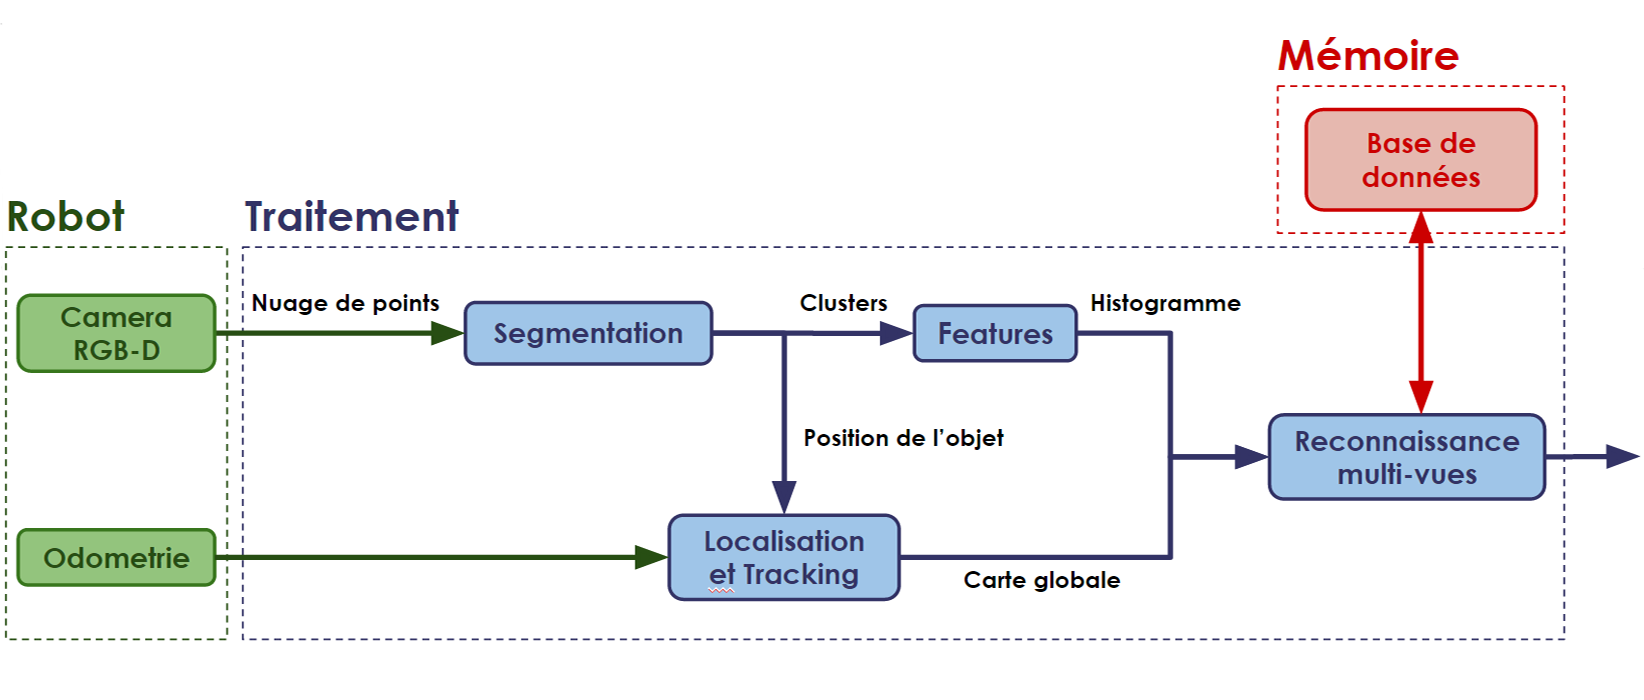
\includegraphics[width=0.95\textwidth]{gen_arc.png}
  \caption{Architecture générale du système}
  \label{fig:architecture}
\end{figure}

Plus précisément, l'unité de traitement reçoit un nuage de points brut provenant de la caméra, ainsi que la mesure de rotation de roues du robot. La première partie du traitement vise à nettoyer le nuage en segmentant des points des objets candidats de la scène, ce qui permet d'enlever une partie non pertinente et de créer un nuage de point dédié pour chaque objet de l'image. Ces nuages de points sont envoyés à l'unité d'extraction de features pour générer des histogrammes représentatif de chaque objets dans l'image. Simultanément, une conversion de référentiel localise des objets dans le repère absolu de déplacement du robot. Puis, les positions des objets sont données au module de localisation et tracking qui suit les observations et les associes entre elles pour avoir une cohérence globale des positions. En dernier lieu, pour chaque objet, les histogrammes de features ainsi que leurs positions converties dans un repère global sont envoyées au module de reconnaissance, et sont utilisés pour reconnaitre les éléments de la scène et donner leur vue la plus probable à chaque instant de temps. 

Les prochaines sections détaillent l'architecture présentée à l'image \ref{fig:architecture}, en présentant le fond théorique derrière le fonctionnement de chaque sous-module.

\section{Segmentation}

La segmentation consiste à isoler des objets dans une image brute, ou en d'autres termes, différencier les éléments qui ne constituent pas un objet et les objets eux-mêmes. La segmentation d'objets est considérée comme un élément essentiel en traitement d'image étant donné qu'une fois l'objet séparé du fond, la reconnaissance devient beaucoup plus simple. La difficulté majeure d'un tel algorithme sur des images RGB vient du fait que la projection de la scène sur le plan image supprime l'information de profondeur. Les capteurs stéréoscopiques et infra-rouges permettent de compenser cette absence d'information et simplifient énormément le traitement nécessaire.

Dans le cas où le capteur est immobile, on utilise classiquement des méthodes de soustraction de fond pour l'étape de segmentation \cite{dai2006prospects}. Ceci n'est pas possible dans notre cas car le robot évolue dans son environnement. La démarche proposée par la littérature dans ce cas considère les objets comme des ensembles de points délimités par un seuil de proximité. Cette définition est suffisamment générale pour permettre de représenter une grande quantité d'objets. Néanmoins, définir ces ensembles dans une image brute n'est pas forcément simple. Par conséquent, on utilise un nouvel \textit{a priori} qui spécifie que les objets se situent sur des plans de support. Bien que plus restrictif que la définition d'avant, cela permet un segmentation crédible. Parmis les méthodes de segmentation se basant sur cette définition, on peut citer Tabletop object detector \cite{tabletop} qui détermine le plan principal de l'image (généralement une table ou le sol) grâce à l'algorithme RANSAC \cite{fischler1981random}, puis recherche des objets dans l'enveloppe convexe de ce plan. Par ailleurs, Caron et al. \cite{caron2014neural} ont proposé une approche légèrement différente. En partant du même principe, le sol est estimé, puis un traitement pour le fond de la scène est appliqué, où les plans orthogonaux à la normale du sol et de taille suffisamment grands sont considérés comme des murs, et les éléments trop près des bords ne sont pas considérés. 

\subsection{Algorithme}

La méthode de segmentation utilisée dans notre cas est celle proposée par Caron et al. Cette méthode s'applique surtout pour de la segmentation d'objets posés sur le sol dans des environnements intérieurs et répond aux exigences du domaine de déplacement du robot : le laboratoire de Thales Theresis.\\

Plus spécifiquement, elle peut être découpée selon les étapes suivantes :
\begin{enumerate}[start=0]
\item Calibration permettant d'obtenir l'équation du sol avant le début de la séquence. Puis, pour chaque frame de la séquence
\item Soustraction du sol à partir de l'équation trouvée
\item Filtrage des points trop éloignés, considérés comme plus incertains
\item Calcul de la normale des surfaces de la scène
\item Élimination de murs, considérés comme des plans orthogonaux au sol et de taille suffisamment grande
\item Voxelisation des points non filtrés pour accélérer le traitement
\item Projection des points voxelisés dans le plan du so
\item Regroupement des points en objets grâce à l'algorithme de \textit{clustering} point growing de PCL
\item Calcul du centroïde et des bounding boxes 2D et 3D de chaque objet
\end{enumerate}

Ainsi, l'algorithme fournit la position de chaque objet dans le repère de la caméra ainsi que le nuage de point et les normales qui leur sont associés.

Une calibration initiale est nécessaire pour définir l'équation du sol. Pour cela, on place le robot dans un endroit où l'image obtenue correspond majoritairement au sol. L’équation du plan dominant est extrait par RANSAC et sauvegardée dans un fichier texte. Une explication plus détaillée sur les sous-méthodes utilisées pour chaque étape est présentée dans les annexes, ainsi qu'une discussion sur les paramètres utilisés.


\subsection{Restrictions} 
\celine{Ce paragraphe aurait peut être plus sa place dans les annexes. Vois en fonction de la place qu'il te reste ...}
La physique des capteurs restreint le type d'objets qui peuvent être aperçus et segmentés, soit à cause des réflexions des rayons infra-rouges, soit à cause de la
résolution limitée des images mesurées. D'un autre côté, la segmentation a ses propres contraintes en ce qui concerne le positionnement des objets dans l'image et, principalement, la définition du sol et des murs. Par conséquent, les restrictions de l'algorithme sont les suivantes :

\begin{itemize}
\item L'objet se trouve par terre.
\item L'objet se trouve au centre de l'image.
\item La lumière ambiante ne doit pas contenir trop de lumière infra-rouge.
\item L'objet n'est ni transparent ni trop réflectif.
\item Le sol où le robot se déplace n'est pas accidenté.
\item L'objet se trouve à une distance inférieure à 3 mètres.
\item L'objet est assez grand et dépasse le seuil d'appartenance au sol.

\end{itemize} 

Un grand nombre d'objets, entre autres chaises, tables, écrans, boîtes en carton, poubelles, de tailles et formes variés ont été testés et peuvent être segmentés malgré les restrictions. Quelques exemples de segmentation sont présentés en annexes \ref{annexe:segmentation} pour illustrer la capacité de segmentation. \celine{Si tu as de la place, tu peux carrément montrer des exemples dans cette section et non dans les annexes.}

\section{Descripteurs}

Le travail des descripteurs est, d'une part, d'extraire des caractéristiques intéressants de l'élément observé et, d'autre part, de réduire la
dimensionnalité de l'espace traité, tout en restant robuste à des transformations affines et aux changements de luminosité. On s'intéresse surtout ici aux descripteurs basés sur le nuage de point des objets, bien qu'il soit possible aussi d'utiliser des descripteurs associés à la texture ou à la couleur. Les descripteurs qui nous intéressent sont des descripteurs géométriques qui essaient de traduire les idées de courbure, de forme et taille dans les histogrammes, et sont intéressants pour étudier les ambiguïtés de reconnaissance. Parmis les descripteurs 3D proposés dans la littérature, on peut citer FPFH \cite{rusu2009fast} qui est invariant par changement de point de vue, SHOT \cite{tombari2010unique} étant un descripteur local de courbure et des descripteurs semi-globales orientés au traitement des occlusions CVFH \cite{aldoma2011cad} et Our-CVFH \cite{aldoma2012our}. Une description détaillée de ces descripteurs et leurs principales différences sont expliquées dans les annexes \ref{annexe:descripteur}. Nous choisissons d'utiliser le descripteur \textit{Viewpoint Feature Histogram} - VFH, car il permet de discriminer non seulement les formes géométriques (pour la reconnaissance d'objet), mais aussi les points de vues (reconnaissance de vue).

En partant de l'hypothèse que la segmentation propose un découpage correct des objets, on extrait des descripteurs globaux à partir des ensembles de points proposés. Ainsi, pour chaque objet, on obtient un histogramme VFH représentatif de l'objet et de la vue segmentée.

\section {Reconnaissance mono-vue} 

matching des descripteurs avec la base de données...

L'étape de classification correspond à la différentiation entre les
histogrammes caractéristiques de chaque vue de chaque objet. Cette
mesure pourrait être apprise, par exemple, avec un réseau de neurone
ou n'importe quel autre méthode classique de \textit{machine learning}.{\color{green}Le travail * three dimensional
  dof cluster vfh...* suggère l'utilisation de la mesure chi-squared
  similarité entre histogrammes accouplé au classificateur k plus
  proches voisins. }  Le grand avantage de ce classificateur c'est l'étape
d’apprentissage correspond à création d’un arbre de recherche,
construit d'après la comparaison croisée entre les éléments de la base,
que pour l'ordre de grandeur de la base de données envisagé, est
presque instantané. Distance plus naturel...

\begin{figure}[H]
	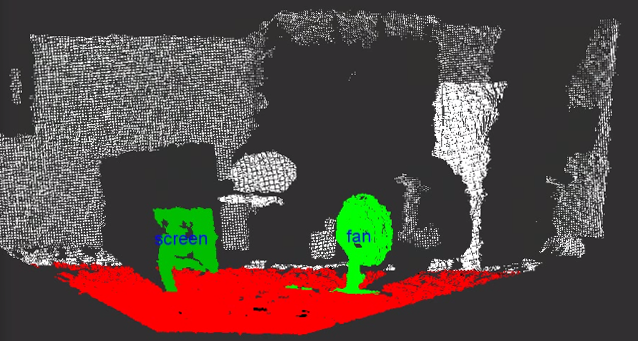
\includegraphics[width=\textwidth]{mono_recon.png}
	\caption{\textbf{reconnaissance mono-vue} - Le résultat de la classification sur les objets segmentés où une écran et un ventilateur étaient reconnus. En rouge le plan du sol et en blanc les points à plus de 3 mètre considérés comme plus bruités. Un remarque pour les ombres infra-rouges qui occultent les objets}   
\end{figure}

L'API de la librairie FLANN sur PCL permet l'utilisation directe du classificateur
K - plus proches voisins. L'implémentation permets l'utilisation de plusieurs
définitions de distance entre histogrammes. La définition par défaut, Chi-squared,
dont la formule est décrit dans la suite, semble être capable de bien différentier
les histogrammes d'entrés, $H_1$ et $H_2$, et était choisi comme la définition pour le classificateur.

$$d(H_1, H_2) = \sum _I \frac{\left(H_1(I)-H_2(I)\right)^2}{H_1(I)} $$

% Une étude des mesures de corrélation entre histogrammes peut être
% intéressant. Ces mesures sont classifié en deux classes : croisés et
% directs. La comparaison direct prend en compté différences par rapport
% à la même cellule de l’histogramme. Pendent que la comparaison croisée
% permet la comparaison entre cellules, par une matrice de
% corrélation. Les features géométriques ont des cellules bien définis
% et statiques, ainsi, semble plus naturel d'utiliser une comparaison
% \textit{bin-to-bin}.
% \subsection{bin-to-bin} Comparaison entres cellules équivalents
% \begin{itemize}
% \item Correlation :
% \item Intersection :
% \item Bhattacharyya distance :
% \end{itemize}

\section{Localisation et suivi d'objet}

\subsection{Définition de repères}

Se placer dans différents repères permettre d'avoir de référentiels plus naturels pour chaque type de composant du robot et pour les objets placés dans la scène. On défini quelques repères et conventions de base pour faciliter la localisation. D'abord le repère de la base du robot est orthonormale positive, où le déplacement vers l'avant correspond à l'axe $x$, vers la gauche à l'axe $y$ et ver le haut à l'axe $z$. Une deuxième référentielle de convention égale à celle d'avant positionne le capteur RGB-D par rapport au robot. Enfin, le dernière référentiel corresponde au repère optique du capteur orienté selon la convention usuelle pour les images avec l'axe $x$ orienté ver la droite et l'axe $y$ ver le bas et, enfin, l'axe $z$ vers l'avant. Ces trois repères permettent d'orienter tous les éléments aperçus par le robot dans l'environnement de façon pratique.

La \review{figure} illustre ces repères utilisés et les conventions décrits.

\subsection{Transformation de repères}

Ensuite, la transformation entre repères permet la passage de l'un à l'autre, pour avoir la position globale de l'objet d'après sa détection par la caméra, par exemple. La transformation entre une base $a$ et une autre $b$ est faite par une matrice de rotation et translation classique, décrit en bas. 

\begin{equation*}
	\mathbf{R}^{a}_{b} = 
	\begin{bmatrix} 
	 	\cos \theta &  -\sin \theta & \Delta x \\ \sin \theta & \cos \theta & \Delta y \\ 0 & 0 & 1
	 \end{bmatrix}
\end{equation*}

où $\theta$ équivaut à la rotation entre les deux repères et $\Delta x$ et $\Delta y$ sont les translations linéaires entre eux.

\subsection{Base mobile}

\subsubsection{Estimation de l'odométrie}

Certains robots sont dotés de capteurs à estimer de façon
approximé sont déplacement. C'est aussi le cas du robot ciblé qui
possède encodeurs capables d'estimer la rotation angulaire des
roues. Pour le cas d'un robot différentiel, où chaque roue peut être
commandée indépendamment, son déplacement et orientation suit les équations suivantes:
\begin{equation*}
	\begin{array}{rcl}
		\delta x_t &=& \frac{\delta \omega_{gauche} + \delta \omega_{droite}}{2} \\
		\delta y_t &=& ...\\
		\delta \theta_t &=& ...								
	\end{array}
\end{equation*}

Une intégration, au sens mathématique, de la différence entre
l'odométrie entre deux intervalles de temps permet de retrouver la
position global du robot.

\begin{equation*}
	\begin{array}{rcl}
		x_t &=& x_{t-1} + \delta x_{t} * cos(\theta_{t-1}) - \delta y_{t} * sin(\theta_{t-1}) \\
		y_t &=& y_{t-1} + \delta x_{t} * sin(\theta_{t-1}) + \delta y_{t} * cos(\theta_{t-1}) \\
		\theta_t &=& \theta_{t-1} + \delta\theta_{t}
	\end{array}
\end{equation*}

\subsection{Filtre de Kalman }

La modélisation des objets entraîne le besoin initiale de les
localiser dans la scène pour, postérieurement, les identifier. À cause
de la divergence de l'odométrie, la mauvaise segmentation et le calcul
du centroïde de l'objet, la position estimée est fortement bruitée
ayant un écart type qui rend la suive et identification infaisable
lorsque plusieurs objets sont minimalement proches. Un filtre de
Kalman ayant un modèle unitaire pour la matrice de transition d'états,
moyenne les observations pour s'adapter au bruit de mesure.

Cependant, le caractère monomodal du filtre de Kalman fait en sorte
qu'un seul objet cible peut être suivis à la fois. Pour atteindre
l'aspect multimodal, il faut que plusieurs filtres tournent en
parallèle. Ainsi, le problème passe d’estimer la position à décider
quelle observation appartient à quel filtre, l'étape
d'identification. Cela se fait à l'aide d'une matrice de corrélation
de distances entre les nouvelles observations et les états courants de
chaque filtre existant. Une solution simplificatrice est d'associer
chaque observation au filtre selon l'ordre de vraisemblance de cette
matrice. Lorsqu’une ambiguïté se produit dans l'étape
d'identification, la classification peut aider à prendre une décision
de mettre un filtre à jour ou, alors, créer un nouveau filtre.

Classiquement le filtre de Kalman est mis à jour dans deux étapes : 

\subsubsection{Prédiction} Une première de prédiction que s'utilise du modèle linéaire $\textbf{F}_{k}$ pour décrire l'évolution des états au long du temps avec son bruit de process, $\textbf{Q}_{k}$, associé et que estime a priori la covariance de l'erreur en $\textbf{P}_{k|k-1}$. Formalisé dans les équations suivantes:

\begin{equation*}
	\begin{array}{ccl}
		\hat{\textbf{x}}_{k|k-1} &=& \textbf{F}_{k}\hat{\textbf{x}}_{k-1|k-1} + \textbf{B}_{k} \textbf{u}_{k-1}\\
		\textbf{P}_{k|k-1} &=& \textbf{F}_{k} \textbf{P}_{k-1|k-1} \textbf{F}_{k}^{T} + \textbf{Q}_{k}
	\end{array}
\end{equation*}

\noindent Où les variables sont : \\ 
$\textbf{F}_{k}$: dynamique du système \\
$\textbf{u}_{k}$ : entrée de commande \\
$\textbf{B}_{k}$ : matrice qui relie l'entrée de commande u à l'état x \\ 
$\textbf{P}_{k|k-1}$ : matrice d'estimation a priori de la covariance de l'erreur \\
$\textbf{Q}_{k}$ : matrice de covariance du bruit de process

\subsubsection{Innovation}
Une deuxième de mise à jour, où l'observation est incorporé pour le calcule de l'innovation, $\tilde{\textbf{y}}_{k}$, e du gain de Kalman, $\textbf{K}_{k}$.

\begin{equation*}
	\begin{array}{ccl}
		\tilde{\textbf{y}}_{k} &=& \textbf{z}_{k} - \textbf{H}_{k}\hat{\textbf{x}}_{k|k-1} \\
		\textbf{S}_{k} &=& \textbf{H}_{k}\textbf{P}_{k|k-1} \textbf{H}_{k}^{T}+\textbf{R}_{k} \\
		\textbf{K}_{k} &=& \textbf{P}_{k|k-1}\textbf{H}_{k}^{T}\textbf{S}_{k}^{-1} \\
		\hat{\textbf{x}}_{k|k} &=& \hat{\textbf{x}}_{k|k-1} + \textbf{K}_{k}\tilde{\textbf{y}}_{k} \\
		\textbf{P}_{k|k} &=& (I - \textbf{K}_{k} \textbf{H}_{k}) \textbf{P}_{k|k-1}
	\end{array}
\end{equation*}
\noindent Avec: \\
$\textbf{z}_{k}$ : observation ou mesure du process à l'instant k \\
$\textbf{H}_{k}$ : matrice qui relie l'état $\textbf{x}_{k}$ à la mesure$ \textbf{z}_{k}$\\
$\textbf{P}_{k|k}$ : matrice d'estimation a posteriori de la covariance de l'erreur\\
$\textbf{R}_{k}$ : matrice de covariance du bruit de mesure

\section {Reconnaissance Multi-vue}

\subsection {Chaînes de Markov Cachées}

Le déplacement physique du robot résulte dans une séquence
d'observations, en angles différents, d'un même objet. On exploit
l'information odométrique entre les visualisations pour prédire les
prochaines possibles orientations. De cette manière, l'évolution de la
reconnaissance au long du temps est représenté par un processus
stochastique, dont une modélisation possible correspond à le traiter
de façon discrète dans un espace d'état. Ayant l'apriori que la
dernière image et le dernier déplacement suffisent pour faire cette
prédiction, en respectant, donc, la propriété de Markov de premier
ordre, le processus stochastique est modélisée sur le cadre d'une
chaîne de Markov cachée.

Concrètement, les états cachées correspondent à des objets connus au
préalable et déjà incorporés dans la mémoire du robot. Cela contraint le
nombre d'états et on se rencontre avec un chaîne fini. Puis, une
matrice de transition, $a_{i,j}$, décrit l'évolution du processus et c'est là où
l'odométrie et la relation entre vues et entre objets sont
incorporés. Finalement, une autre matrice, $\mathrm{P}\big( y_1 \ | \ k \big)$
, dit matrice d'émission, estime la vraisemblance entre l'observation
et les états de la chaînes.

Une autre deuxième modélisation serait d'avoir une chaîne de Markov
Cachée distincte pour chaque objet et ensuite décider quel était le
processus le plus vraisemblable. Ce cas est un sous-ensemble du cas
antérieur où les transitions entre deux objets ne sont pas
considérés. Pourtant, ce qui peut être utile s'on considère
l'évolution d'objets, par exemple, la transition entre une chaise vide
et une personne assise sur une chaise ou encore un personne
commence à marcher \footnote{Le fait de se mettre en mouvement
  altère les formes d'une personne, ce qui possibilite sa détection
  comme un nouveau objet.}.
  
transition

La variation angulaire entre deux positions du robot est donnée par la relation suivante :
\begin{equation*}
\begin{array}{rcl}
  \vec{d}_0 &=& p_0 - p_{obj}\\
  \vec{d}_1 &=& p_1 - p_{obj} \\
   \delta_{angle} &=& atan(\vec{d}_1) - atan(\vec{d}_0)
\end{array}
\end{equation*}
Ce $\delta_{angle}$ est utilisé pour calculer la transition entre états possibles.

%	mod\(mod\(a,2pi\) + 2pi, 2pi\)
%	angle_wrap\(angle_s1 - angle_s2\) < delta_angle * densité de vue de l'objet = 1
%	0.1 else
%emission
%	\sum_i\(scores\) - scores / \sum_j \sum_k(scores) - scores\)

\subsection{Algorithme de Viterbi}

Il reste, donc, extraire des informations de la modélisation Markovienne proposée.
La séquence d'états la plus vraisemblable qui pourraient avoir géneré
les observations  $y_1,\dots, y_T$, correspondrait exactement à la séquence d'objets reconnus.
A fin de retrouver cette séquence, aussi appéllé chemin, on fait 
appel à la programmation dynamique, spécifiquement à l'algorithme de Viterbi, d'où viens le nom chemin de Viterbi.
L'algorithme retrouve de façon récursive l'état current le plus probable, 
prennant en compte seulement les observations jusqu'au instant donné et son
estimation au instant intérieur, comme décrit par les équations suivants:

\begin{equation*}
  \begin{array}{rcl}
    V_{1,k} &=& \mathrm{P}\big( y_1 \ | \ k \big) \cdot \pi_k \\
    V_{t,k} &=& \max_{x \in S} \left(  \mathrm{P}\big( y_t \ | \ k \big) \cdot a_{x,k} \cdot V_{t-1,x}\right)
  \end{array}
\end{equation*}

La probabilité que la séquence d'états le plus probable finissant dans l'état $k$, avait généré les observation au moment $t$, est sauvegardé dans $V_{t,k}$, pendent que $\pi_i$ c'est la probabilité initiale de se rencontrer en chaque état. Pour retrouver le chemin de Viterbi, il suffit de trouver le maximum de $V_{t,k}$ :

\begin{equation*}
  \begin{array}{rcl}
    x_T &=& \arg\max_{x \in S} (V_{T,x})
  \end{array}
\end{equation*}

\subsection {Graphe d'aspect polaire}

On considère que les objets sont décrits par deux dimensions
d'information : une spatiale, concernant la position absolu de l'objet
dans l'environnement et les positions relatifs où l'objet était
visualisé, et une autre visuelle, donnée par les descripteurs
géométriques, de couleurs et de texture; qu'on cherche à transporter
dans un référentiel unique. Le graphe d'aspect permet de coupler
l'ensemble d'images suivant ses possibles transitions spatiales ce qui
résulte dans la possibilité de construire le modèle à la volée et de
jouer avec sa densité d'information - nombre d'images incorporées.

\begin{figure}[H]
  \centering
  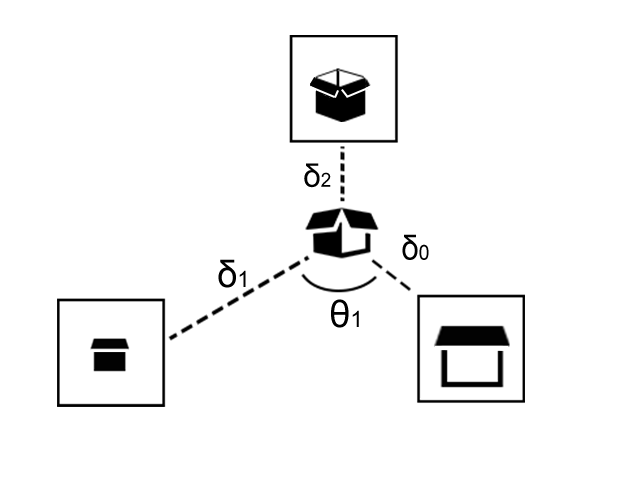
\includegraphics[width=0.4\textwidth]{object_model.png}
  \caption{Modèle polaire des objets.}
\end{figure}

Formellement, un référentiel polaire entrelace toutes ces informations
de façon à représenter la position spatiale d'où l'observation était
fait, tel comme il est représenté dans l'image *7*. Pour la
construction du modèle les conventions suivantes étaient adoptées :
\begin{itemize}
\item l'angle zéro est attribué à la première observation
\item L'origine du référentiel est la position globale de l’objet
\item Les features sont labellisées d'après le déplacement angulaire
  et la distance au centroïde de l'objet.
\end{itemize}

Une grande majorité de features visuelles sont variantes à échelle, une
fois que la résolution de l’image joue un rôle assez critique pour la
détection de features, comme les patches SIFTs. Ainsi, avoir la distance
que l’image étais prise peut être intéressant pour limiter la
classification à une échelle valable.